

\subsection{Closing Plots (Filling the Area Under Plots)}
\begin{command}{\closedcycle}
	Provide |\closedcycle| as \meta{trailing path commands} after |\addplot| to draw a closed line from the last plot coordinate to the first one.
	
	Use |\closedcycle| whenever you intend to fill the area under a plot.

\begin{codeexample}[]
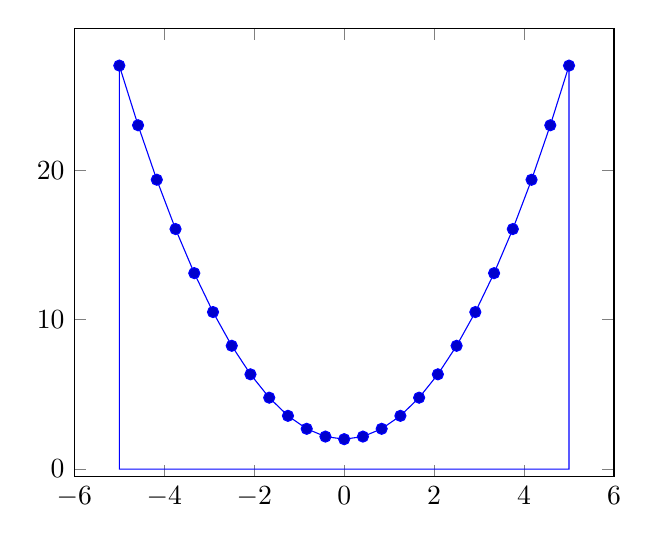
\begin{tikzpicture}
	\begin{axis}
	\addplot {x^2+2} \closedcycle;
	\end{axis}
\end{tikzpicture}
\end{codeexample}

\begin{codeexample}[]
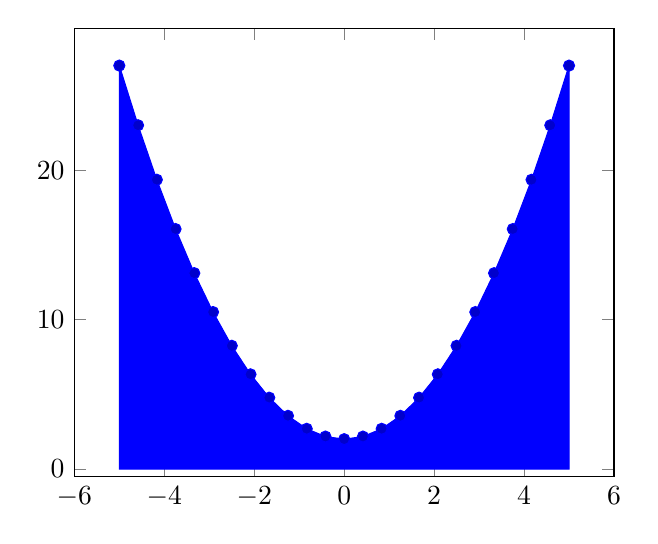
\begin{tikzpicture}
	\begin{axis}
	\addplot+[fill] {x^2+2} \closedcycle;
	\end{axis}
\end{tikzpicture}
\end{codeexample}
	In case of stacked plots, |\closedcycle| connects the current plot with the previous plot instead of connecting with the $x$~axis\footnote{The implementation for stacked plots requires some additional logic to determine the filled area: \lstinline{\\closedcycle} will produce a \texttt{plot coordinates} command with \emph{reversed} coordinates of the previous plot. This is usually irrelevant for end users, but it assumes that the plot's type is symmetric. Since constant plots are inherently asymmetric, \lstinline{\\closedcycle} will use \texttt{const plot mark right} as reversed sequence for \texttt{const plot mark left}.}.
\begin{codeexample}[]
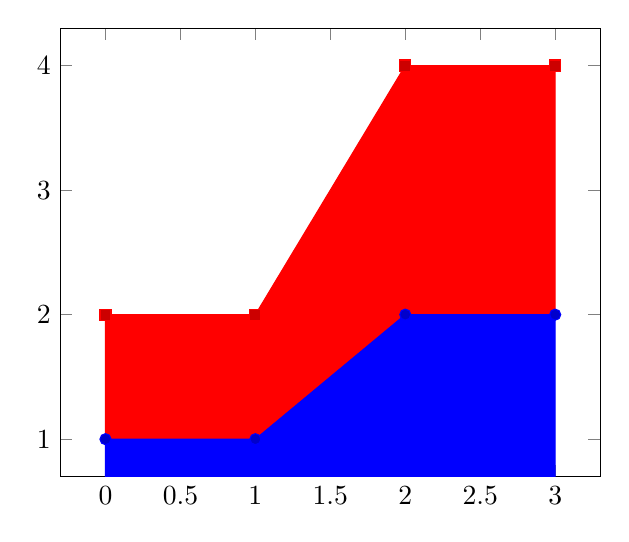
\begin{tikzpicture}
	\begin{axis}[stack plots=y]
	\addplot+[fill] coordinates 
		{(0,1) (1,1) (2,2) (3,2)} \closedcycle;
	\addplot+[fill] coordinates 
		{(0,1) (1,1) (2,2) (3,2)} \closedcycle;
	\end{axis}
\end{tikzpicture}
\end{codeexample}
\end{command}

Note that |\closedcycle| has been designed for functions (i.e.\ for a plot where every $x$ has at most one $y$ value). For arbitrary curves, you can safely use the \tikzname\ path \declareandlabel{--cycle} instead which simply connects the last and the first path element:
\begin{codeexample}[]
\begin{tikzpicture}
	\begin{axis}
	\addplot coordinates 
		{(0,1) (1,2) (0,3) (-1,2)};
	\end{axis}
\end{tikzpicture}
\end{codeexample}

\begin{codeexample}[]
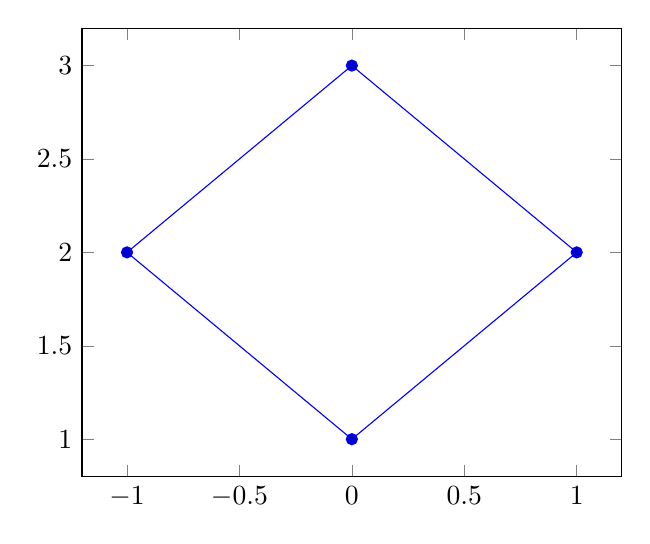
\begin{tikzpicture}
	\begin{axis}
	\addplot coordinates 
		{(0,1) (1,2) (0,3) (-1,2)} --cycle;
	\end{axis}
\end{tikzpicture}
\end{codeexample}

\begin{codeexample}[]
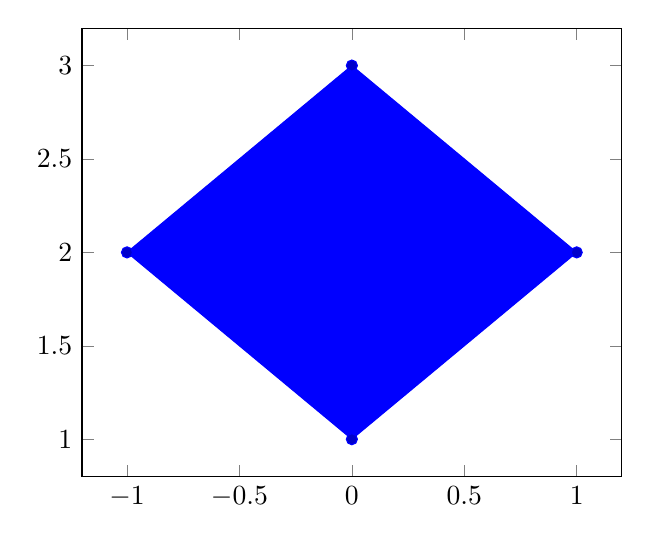
\begin{tikzpicture}
	\begin{axis}
	\addplot+[fill] coordinates 
		{(0,1) (1,2) (0,3) (-1,2)} --cycle;
	\end{axis}
\end{tikzpicture}
\end{codeexample}
The |--cycle| is actually a path instruction of \cite{tikz}; it connects the first and the last coordinate of one path. Note that this is automatically done for |fill|ed paths.
